\documentclass{article}
\usepackage[a4paper, left=3cm, right=3cm, top=3cm, bottom=2.7cm]{geometry}

\usepackage[utf8]{inputenc}
\usepackage{graphicx}
\graphicspath{ {./images/} }
\usepackage{float}
\restylefloat{figure}
\usepackage{circuitikz}
\usepackage[most]{tcolorbox}

\usepackage{etoolbox}
\makeatletter
\providecommand{\subtitle}[1]{% add subtitle to \maketitle
  \apptocmd{\@title}{\par {\large #1}}{}{}
}
\makeatother


\title{
\includegraphics[scale=0.65]{images/ozu.png}\\
\textbf{EE202 - Circuit Analysis}}
\subtitle{Laboratory #3}
\date{Fall 2022}
%\author{Laboratory 1}

\newcommand{\HRule}{\rule{\linewidth}{0.5mm}}

\begin{document}

\begin{titlepage}
\begin{center}

% Top 

\includegraphics[width=0.55\textwidth]{ozu.png}~\\[2cm]

% Title
\HRule\\[0.4cm]
{ \LARGE 
  \textbf{Lab Report for EE202 Circuit Analysis}\\[0.4cm]
  \emph{Laboratory 3}\\[0.4cm]
}
\HRule\\[1.5cm]

% Author
{ \large
  Ömer Faruk Avcı \\[0.1cm]
  \texttt{faruk.avci@ozu.edu.tr}
}

\vfill

%\textsc{\Large Cyprus University of Technology}\\[0.4cm]
\textsc{\large Department of Electrical and Electronics Engineering}\\[0.4cm]


% Bottom
{\large \today}
 
\end{center}
\end{titlepage}



\newpage

%\maketitle

\section{Introduction}
This lab focuses on practical exploration of operational amplifier (op-amp) circuits, including non-inverting and inverting amplifiers, summing configurations, and gain analysis. 
\subsection{Preliminary Work}
\subsubsection{Preliminary Task 1}
\textbf{Gain: 10}
\begin{figure}[h]
  \centering
  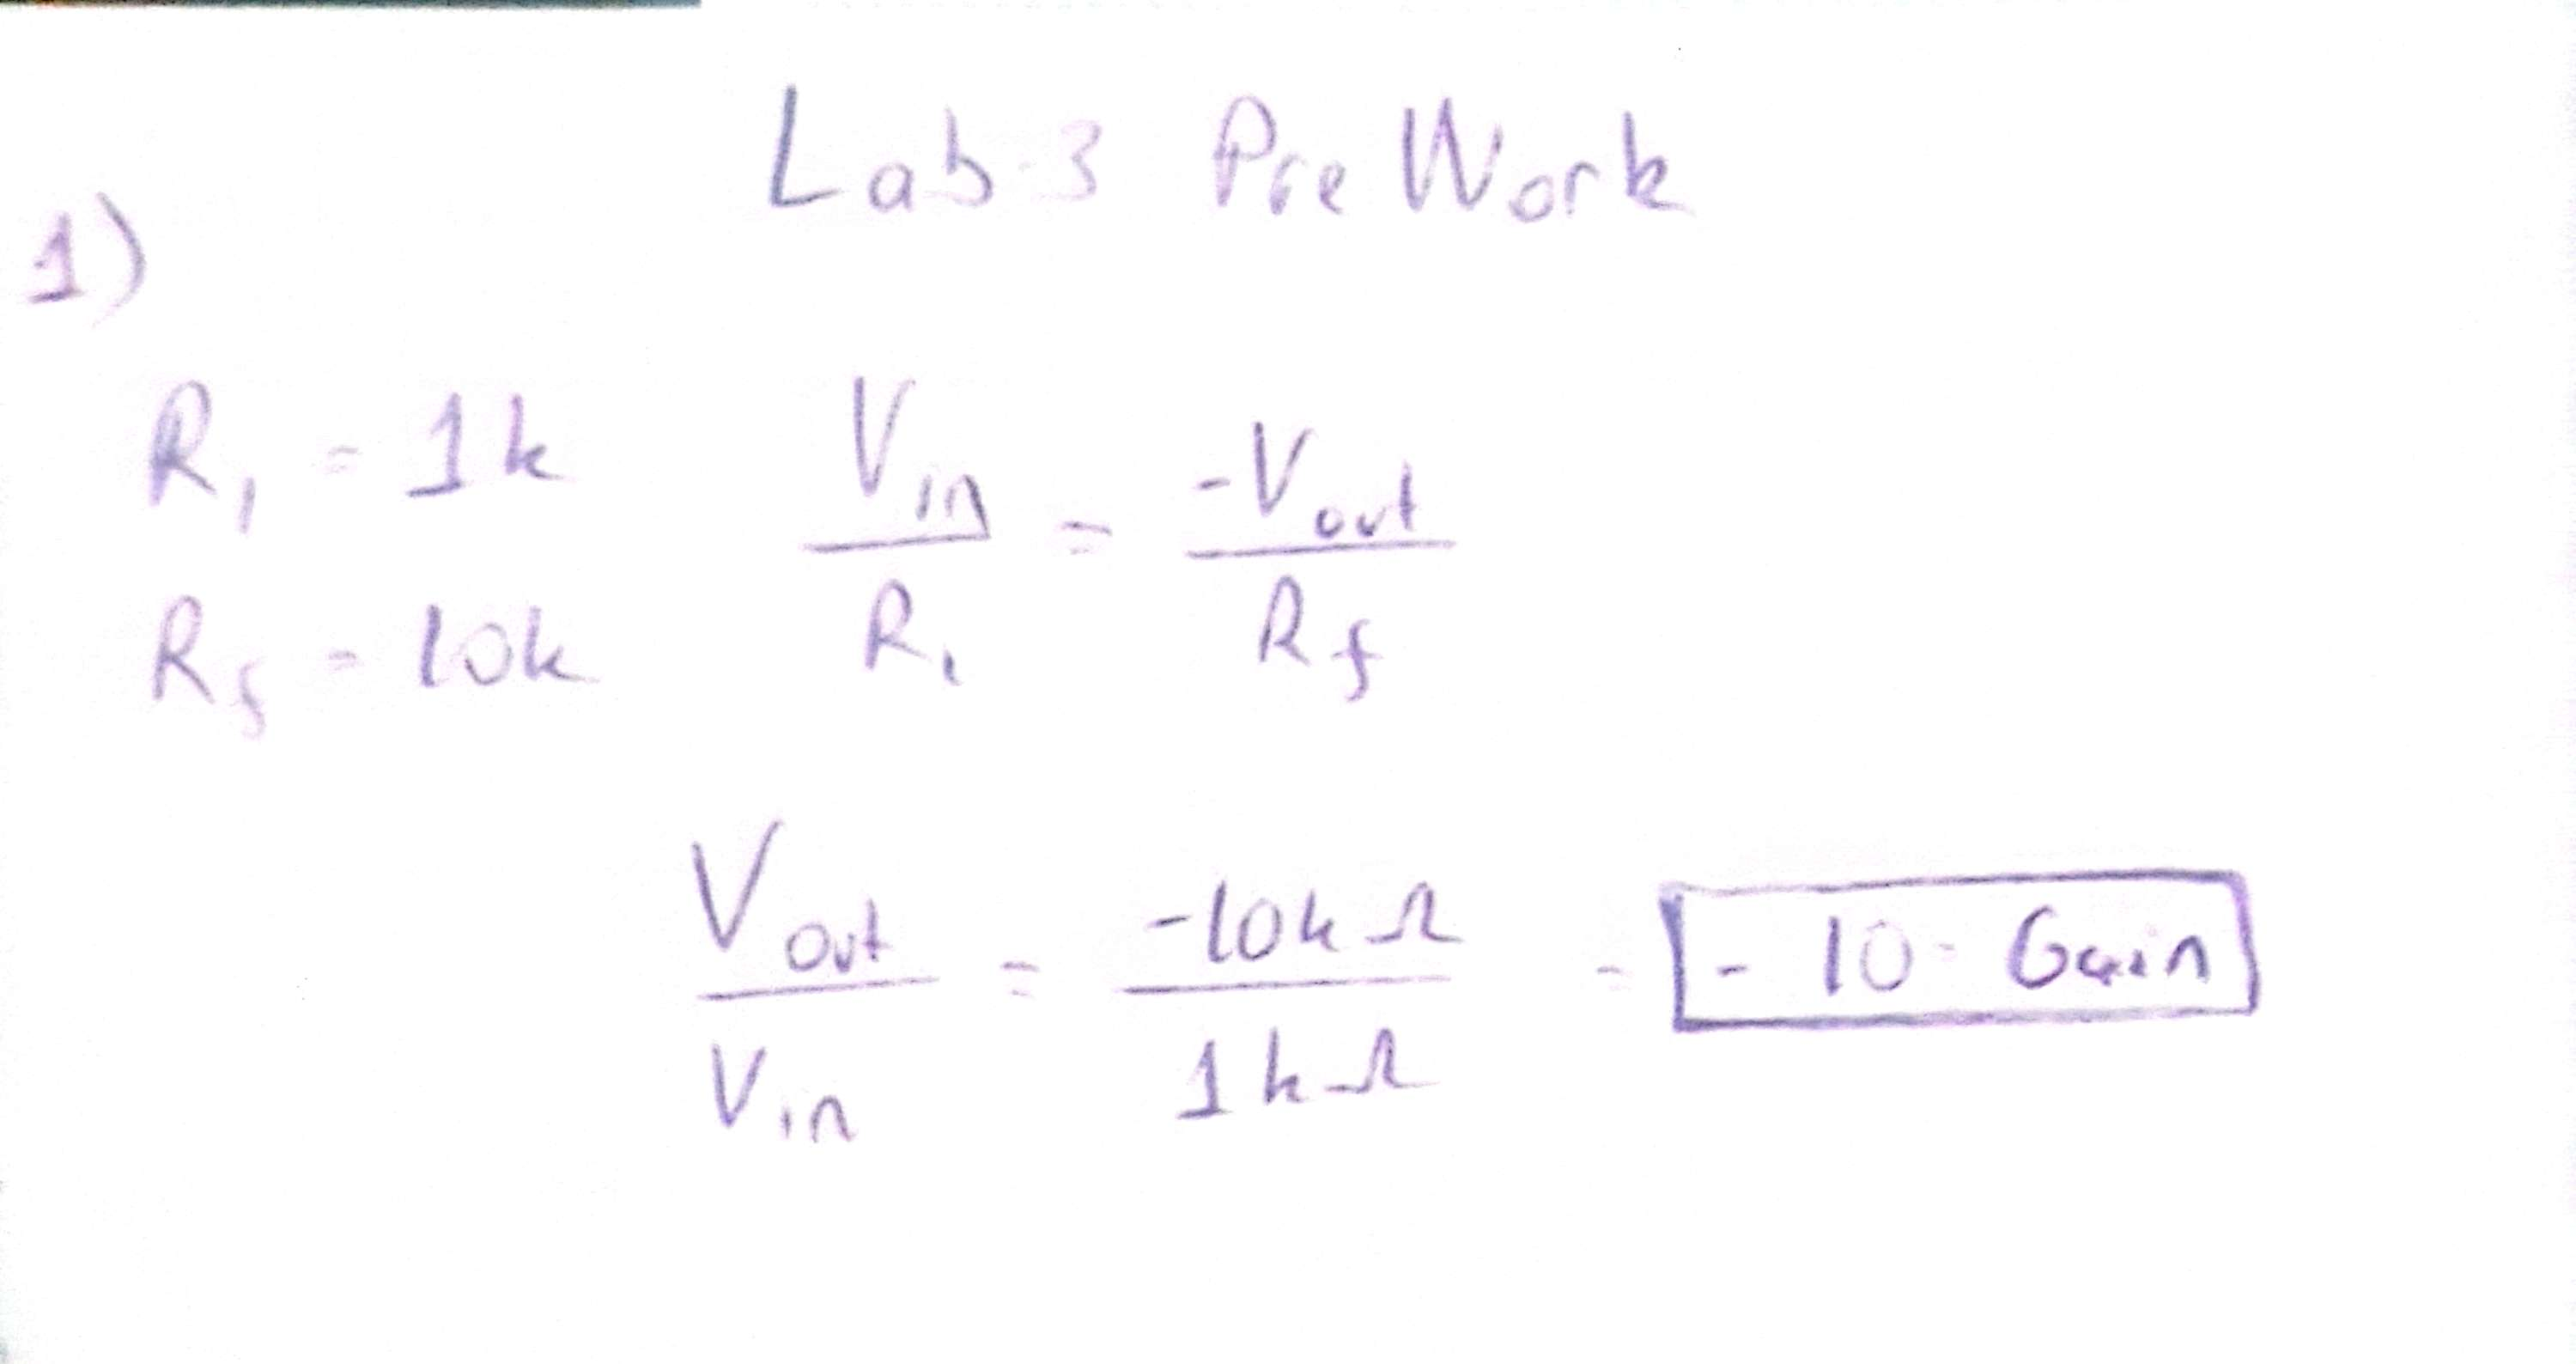
\includegraphics[scale=0.15]{pretask1.jpeg}
  \caption{Inverting op-amp}
\end{figure}

\subsubsection{Preliminary Task 2}
\textbf{$R_f $= 10k}
\begin{figure}[h]
  \centering
  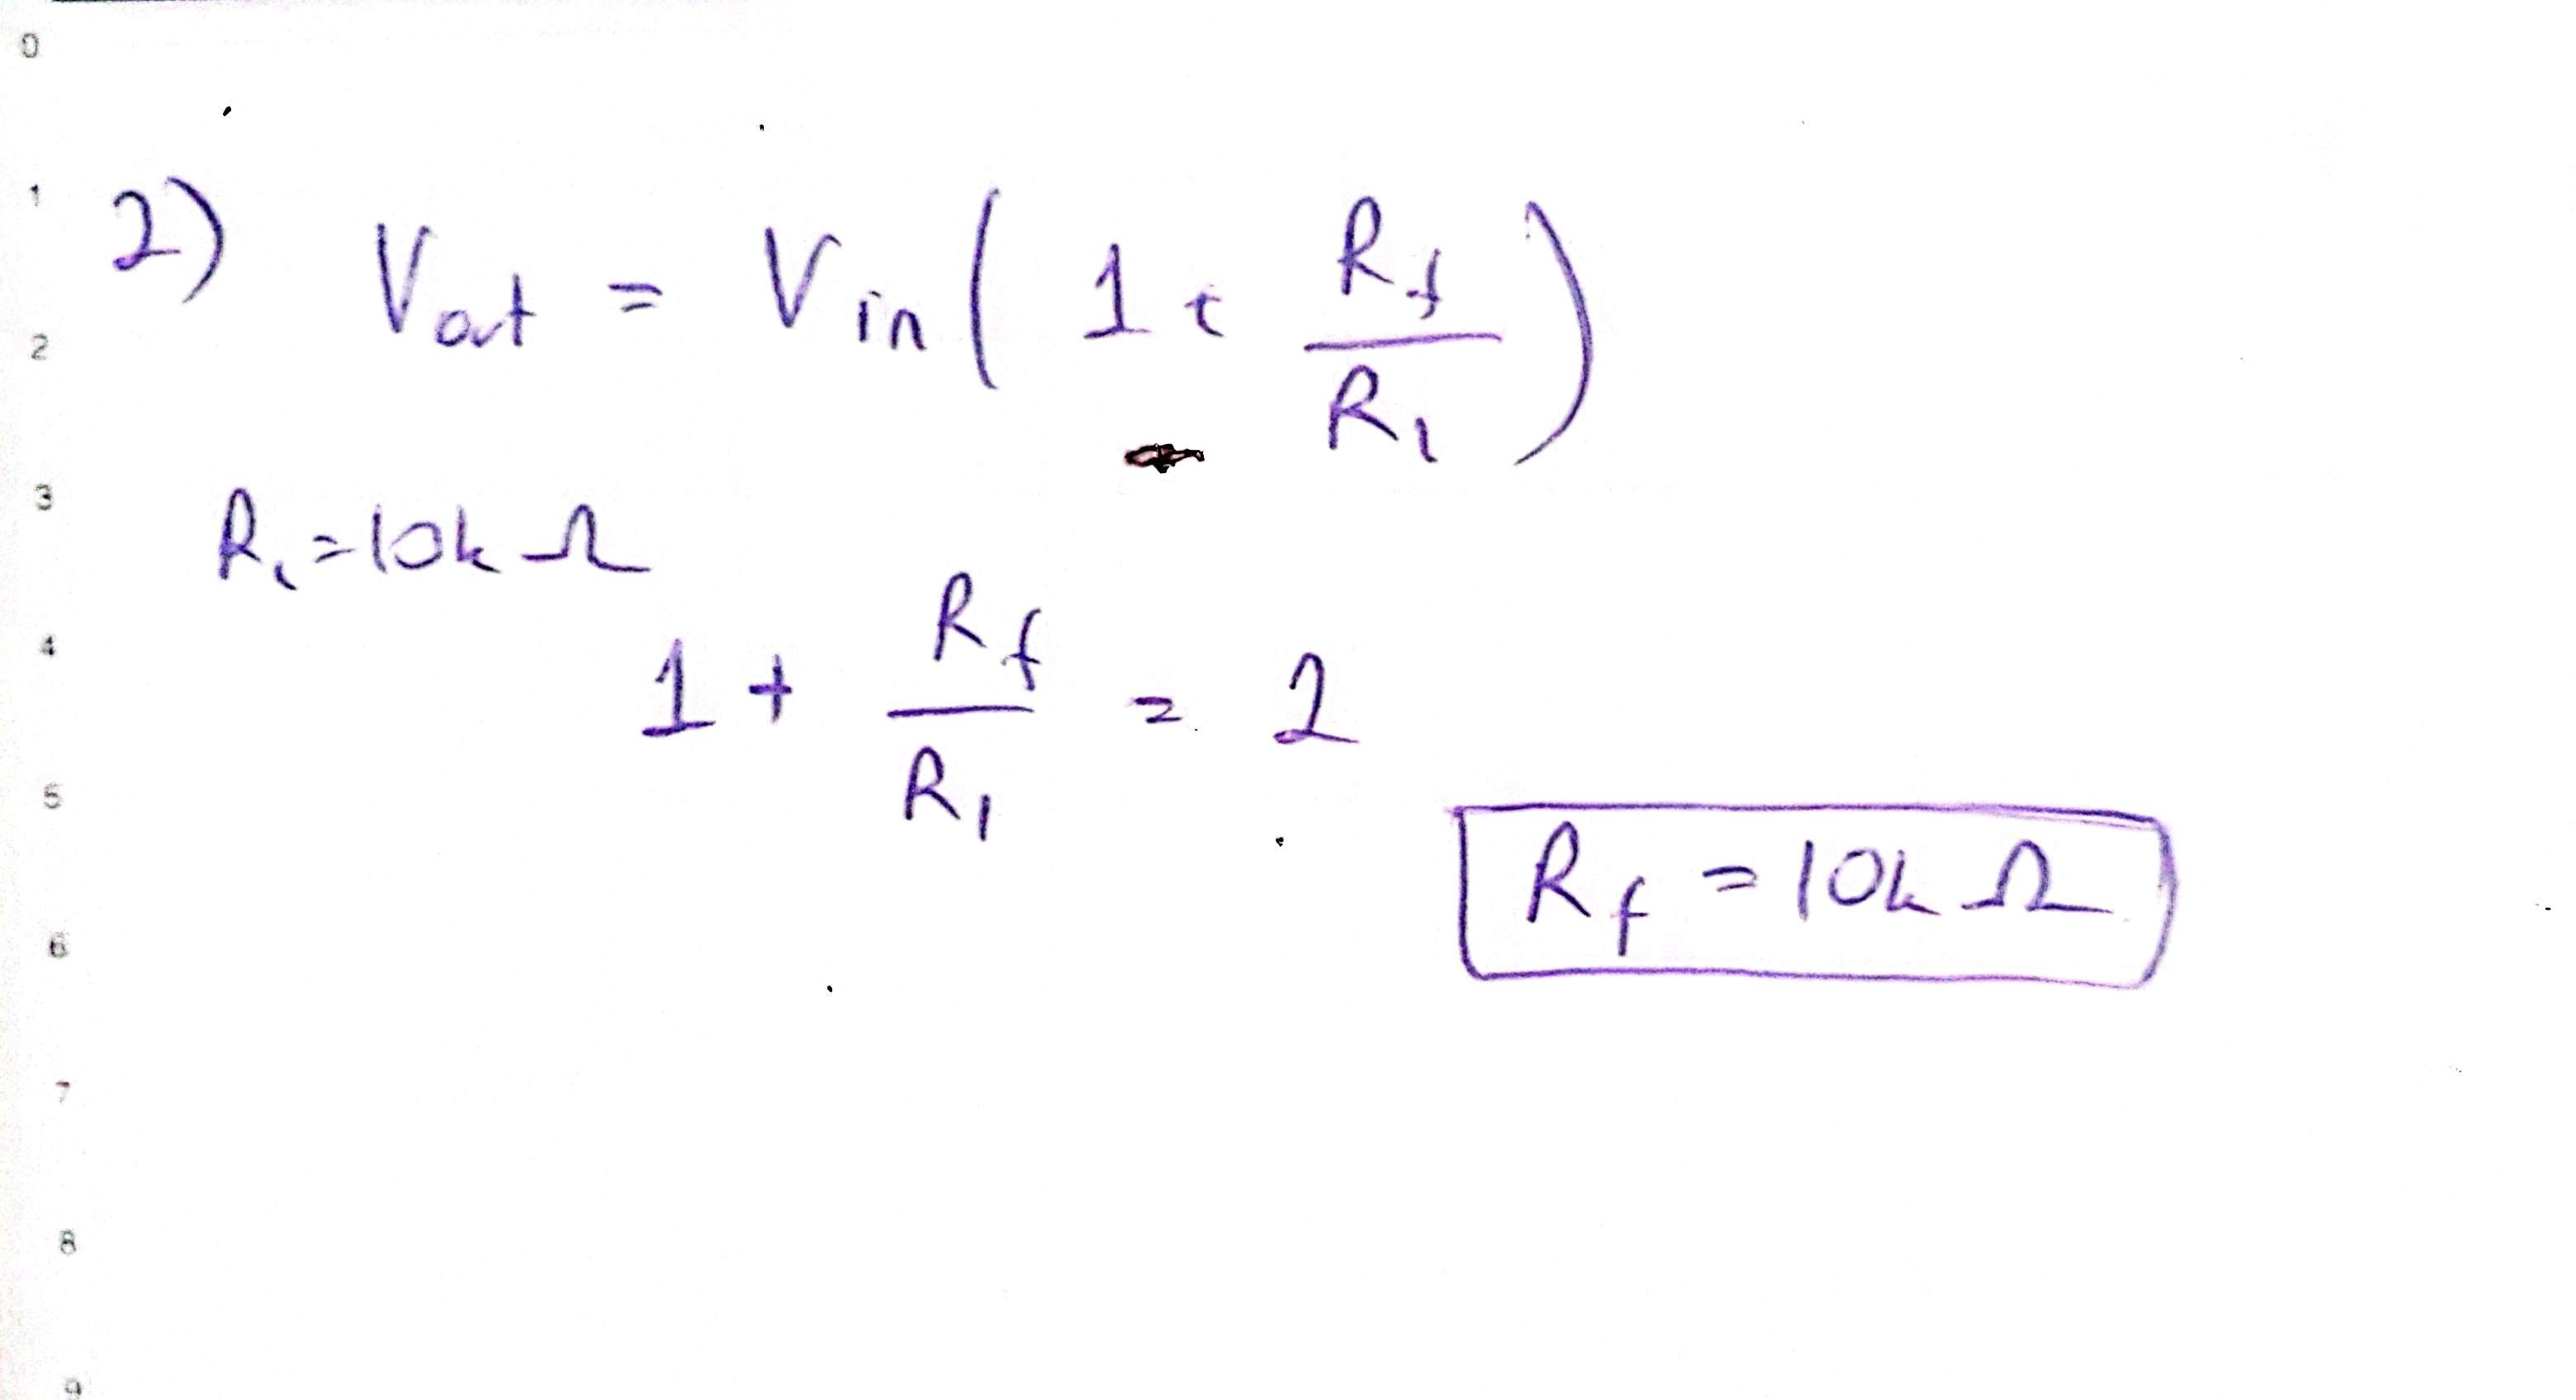
\includegraphics[scale=0.10]{pretask2.png}
  \caption{Inverting op-amp}
\end{figure}



\subsubsection{Preliminary Task 3}
\begin{figure}[h]
  \centering
  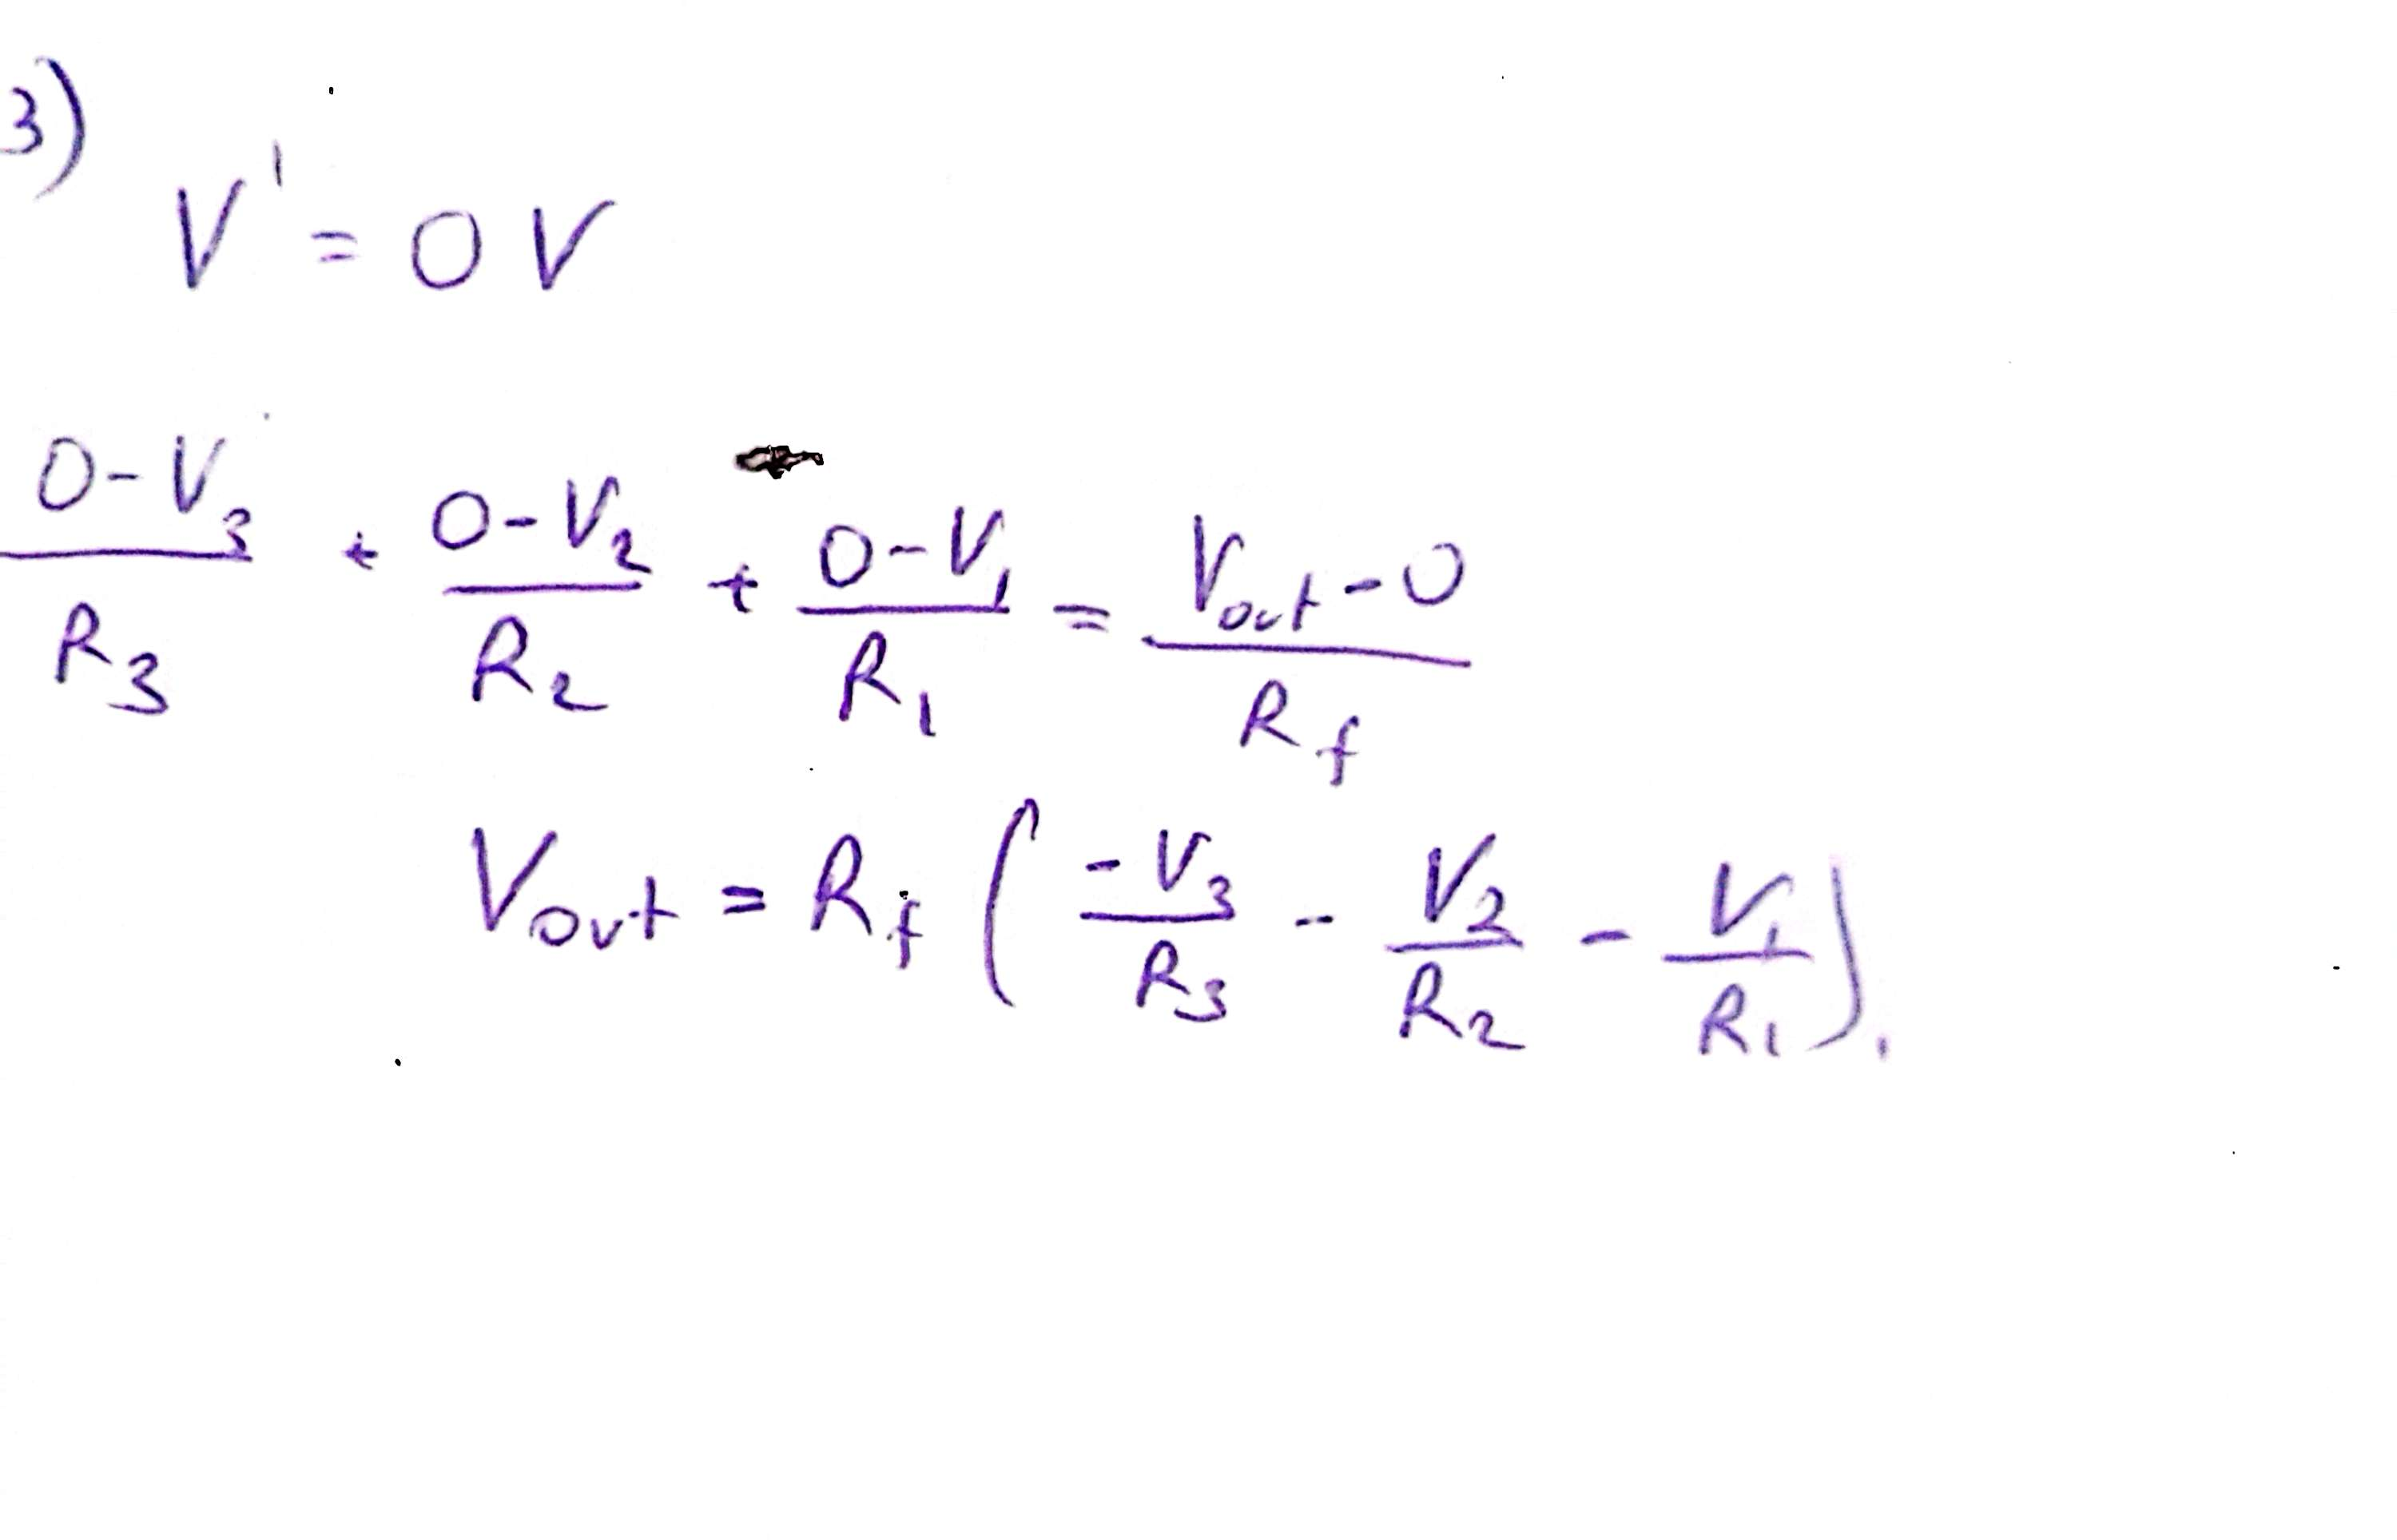
\includegraphics[scale=0.10]{pretask3.png}
  \caption{Summing Amplifier}
\end{figure}



\subsubsection{Preliminary Task 4}
\textbf{Switch on A, Gain = 1}\textbf{; Switch on B, Gain = -1}
\begin{figure}[h]
  \centering
  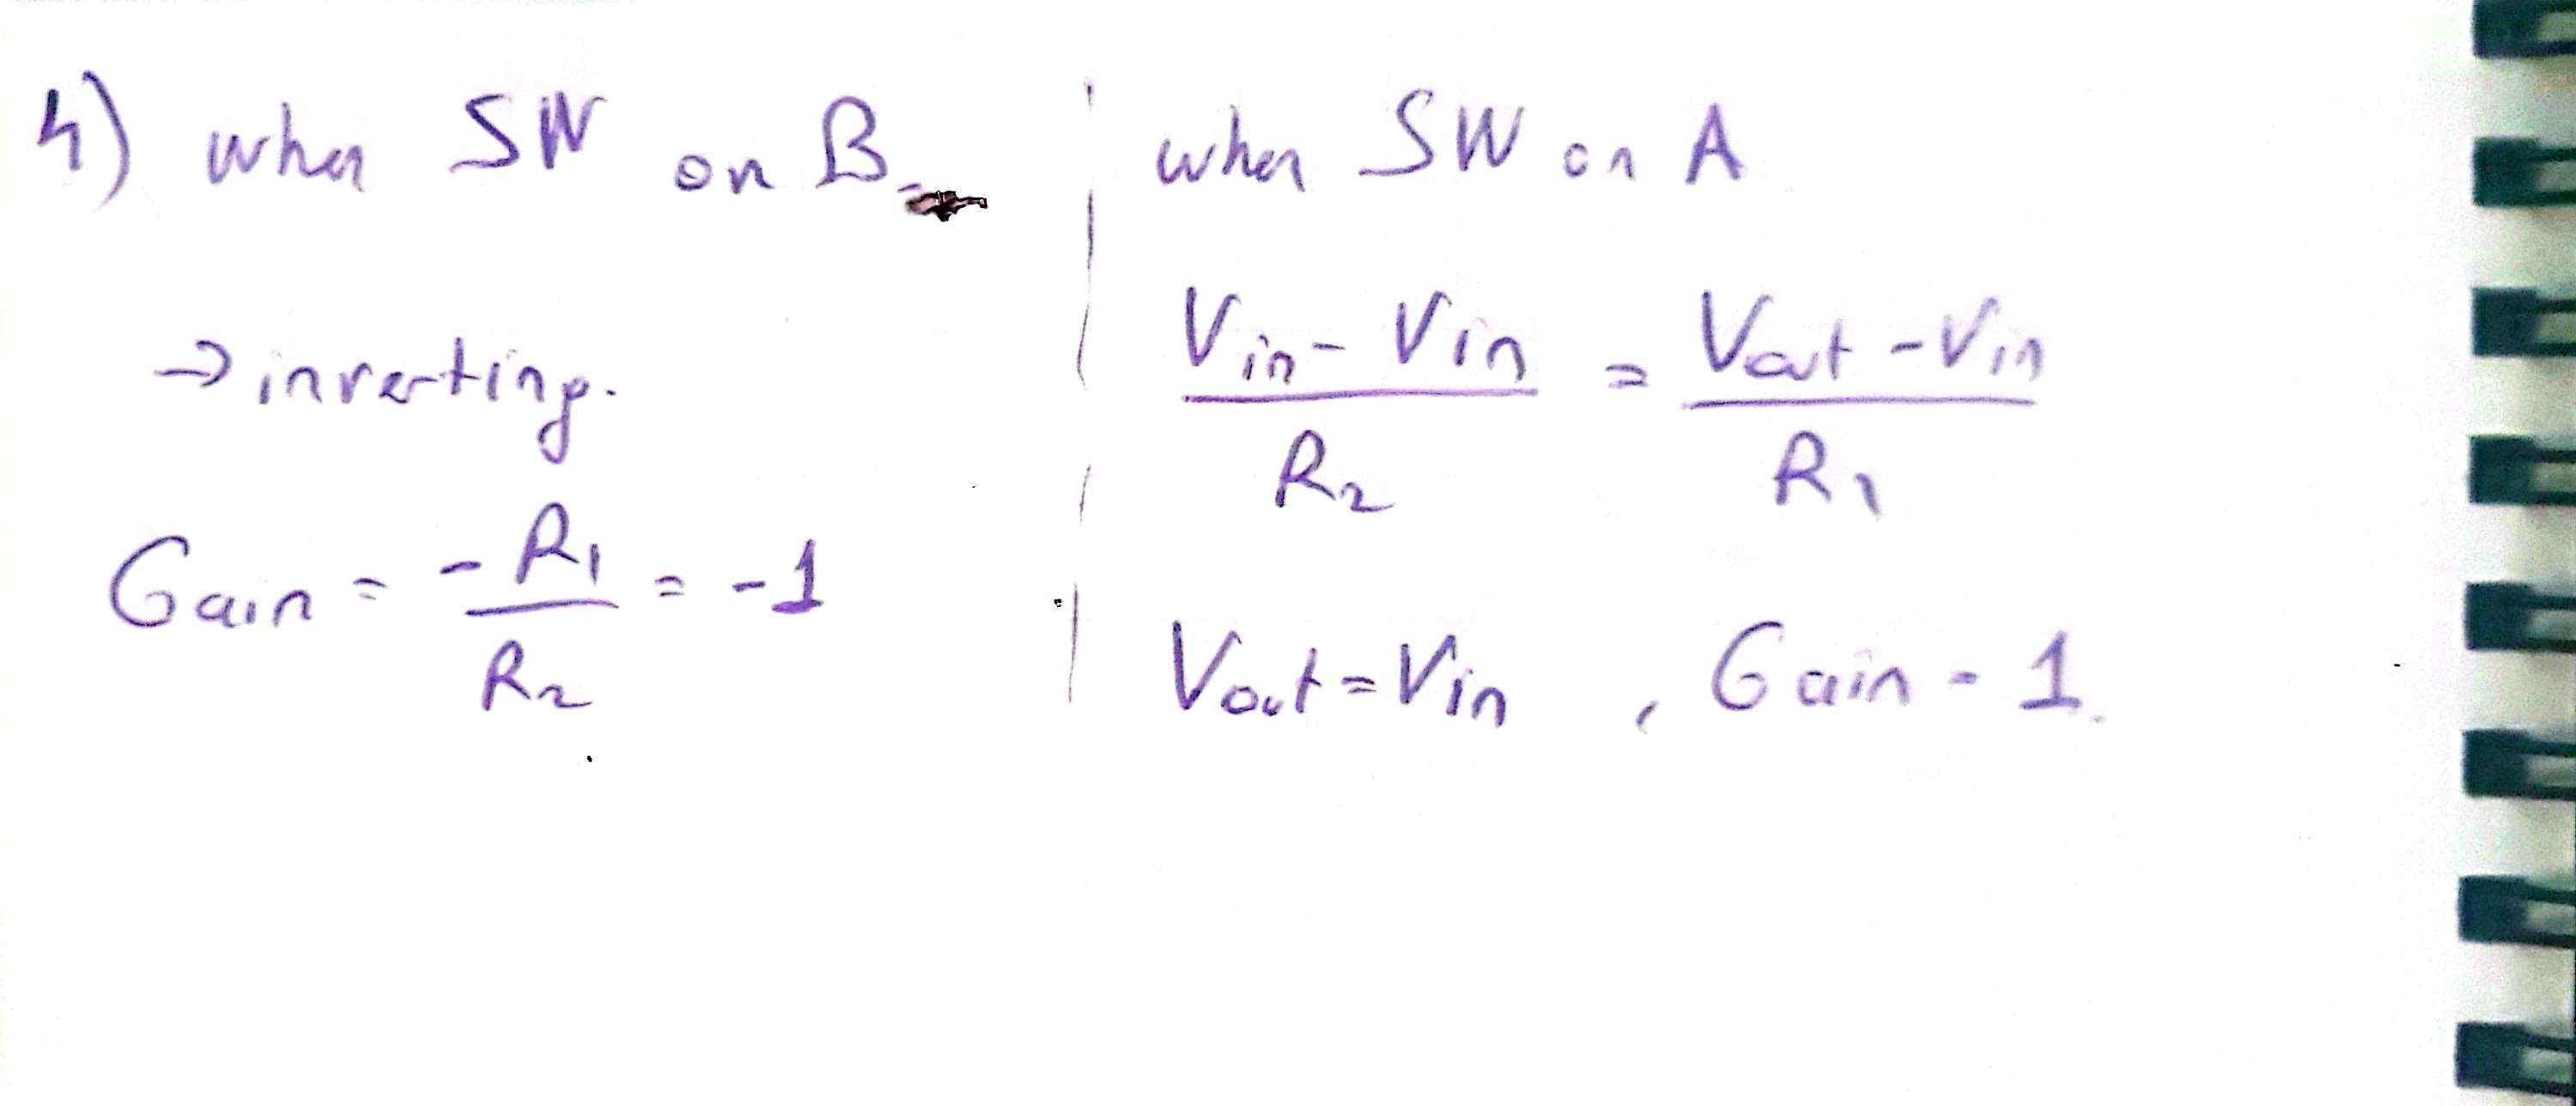
\includegraphics[scale=0.10]{pretask4.png}
  \caption{Op-Amp Consisting of a Switch}
\end{figure}

\newpage

\subsubsection{Preliminary Task 5}
\begin{figure}[h]
  \centering
  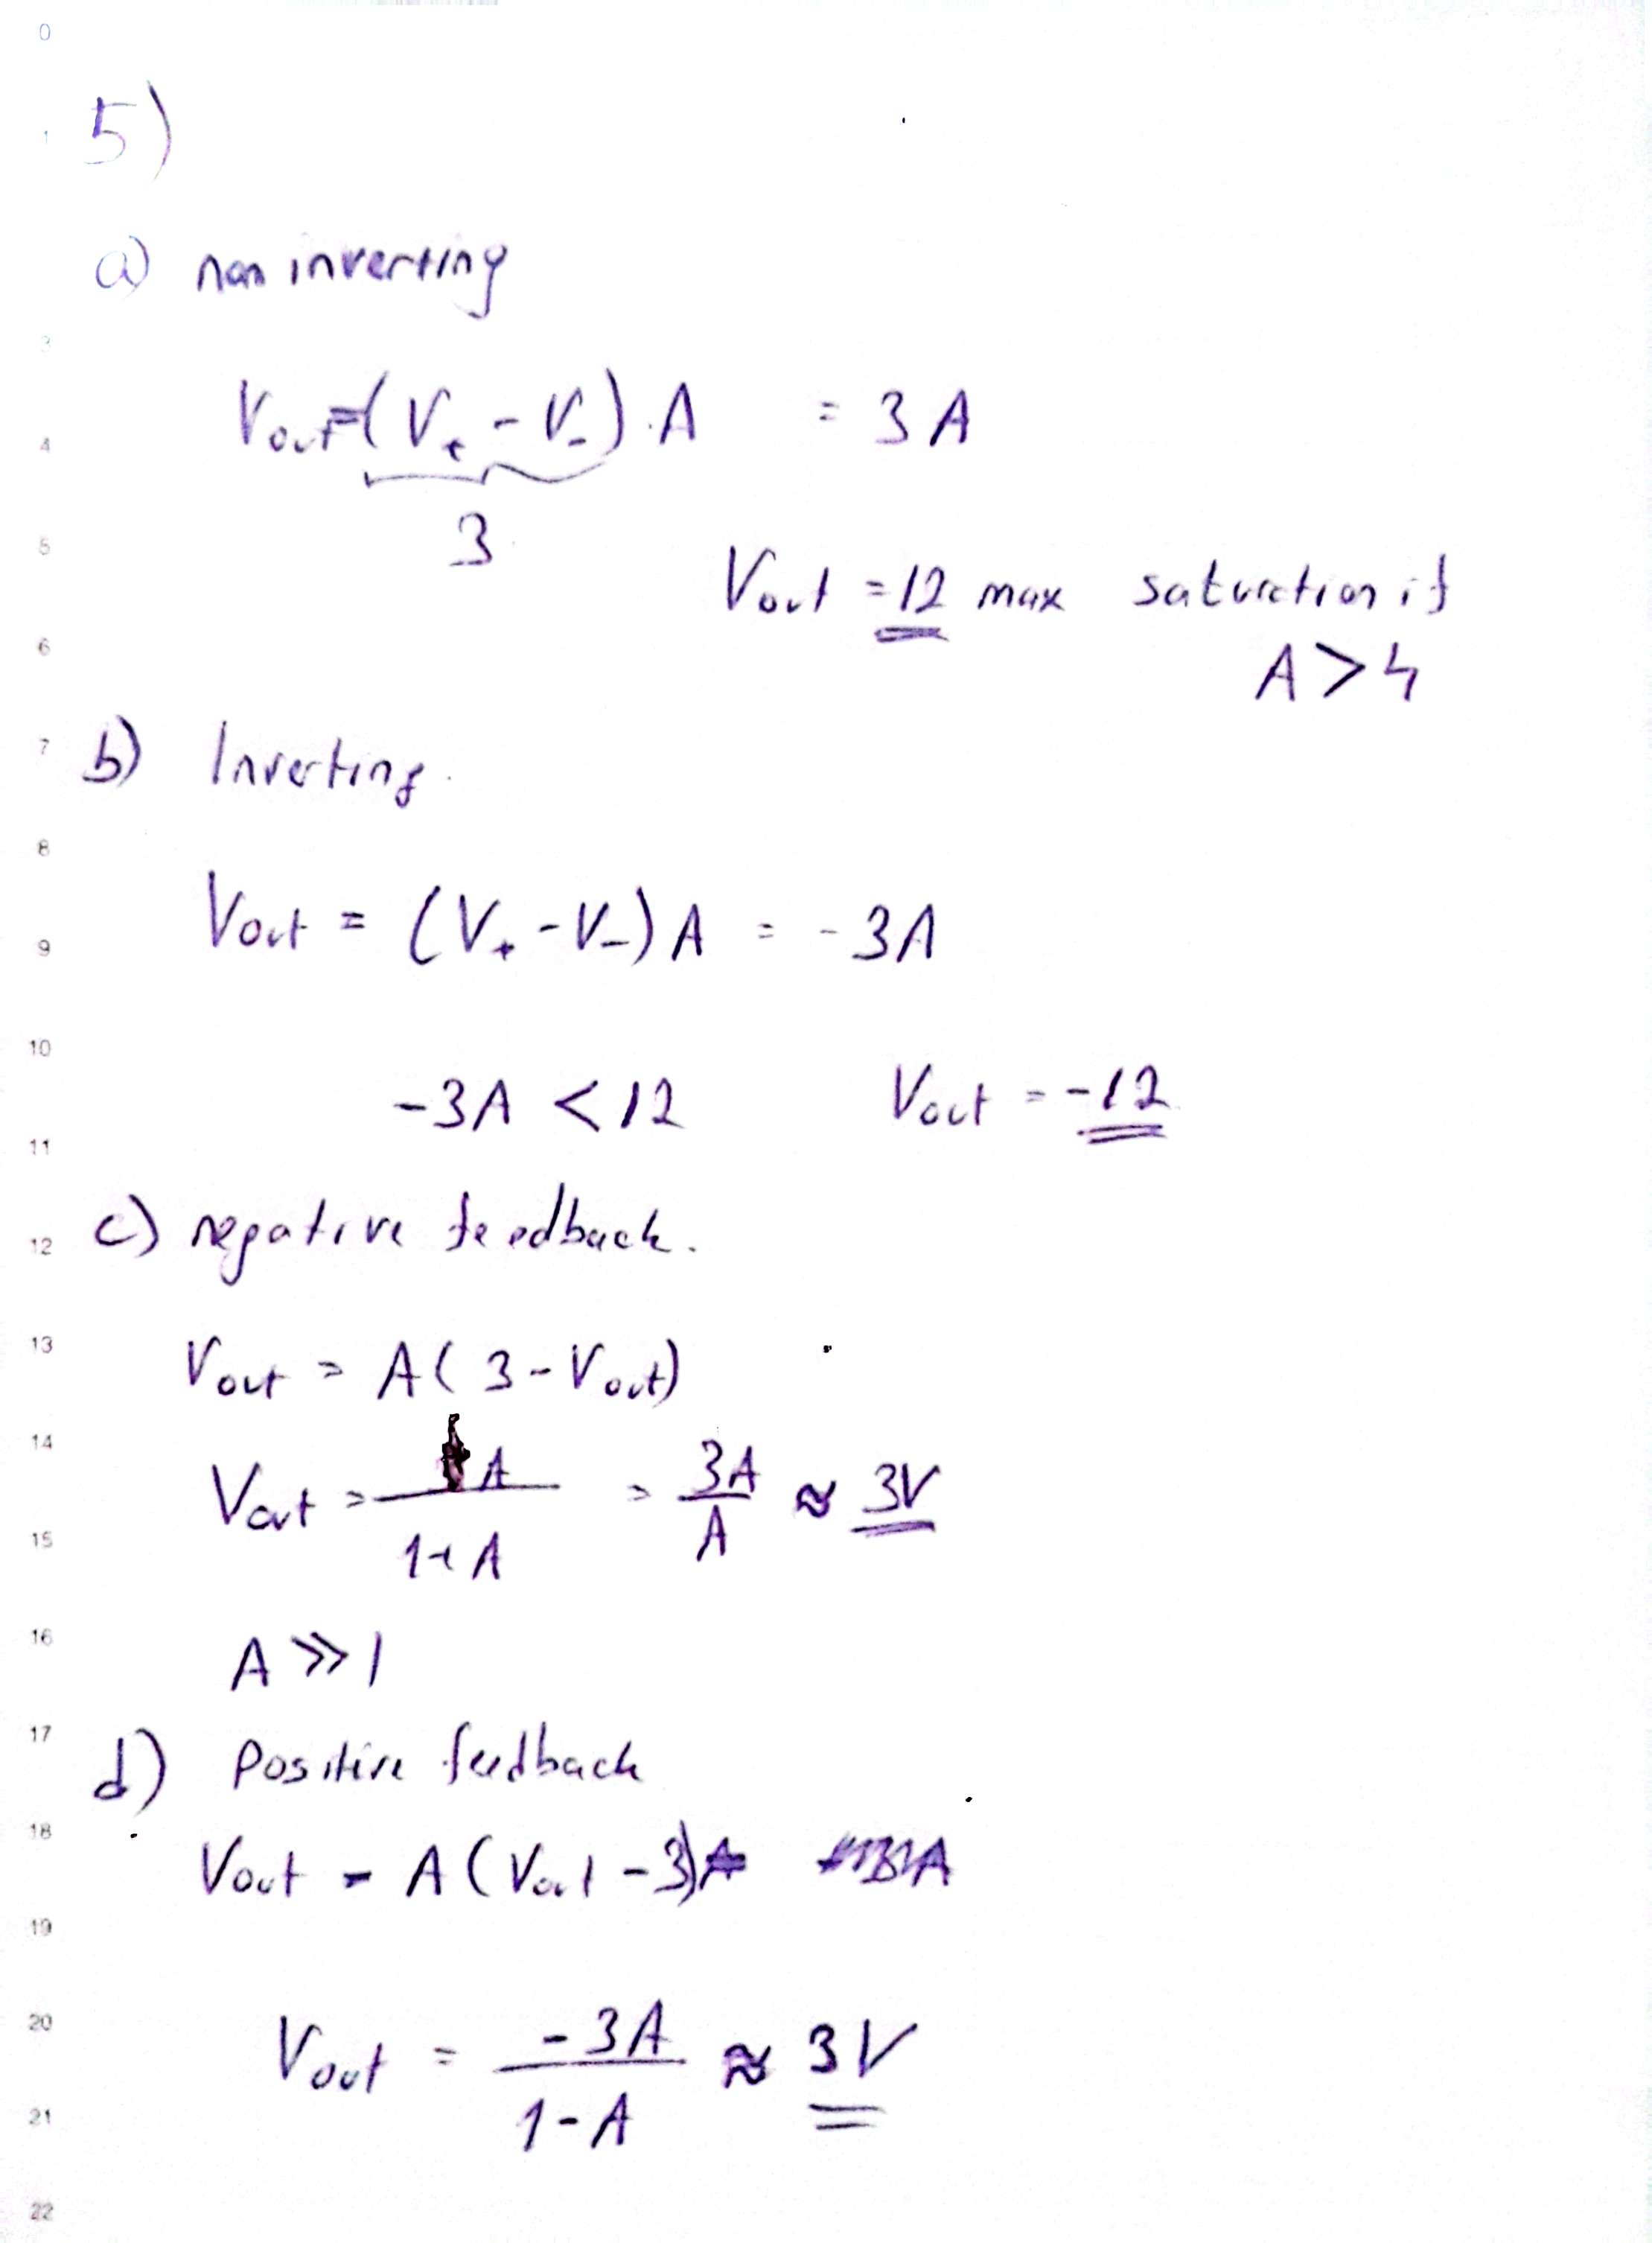
\includegraphics[scale=0.17]{pretask5.png}
  \caption{Op-Amp}
\end{figure}




\newpage
\subsection{Lab Tasks}

In this lab session, we completed 4 different tasks using the uA741 operational amplifier. Each task involved a different circuit setup to explore how the op-amp works.




\begin{tcolorbox}[colback=yellow!15,colframe=black!50!black,title=Important Note]
  Only the pre-lab work is included in this report. Due to time constraints, the lab task sections could not be completed.
  \end{tcolorbox}
  










  
  \begin{center}
  \begin{circuitikz}
  \draw
    (0,0) node[left] {$V_{\text{in}}$} to[R=$R_1$] (2,0)
    (2,0) -- (2,0)
    (2,0) to[R=$R_{\text{f}}$] (4,0)
    (4,0) -- (6,0) node[right] {$V_{\text{out}}$}
    (2,-1) -- (2,1)
    (2,-1) -- (4,0) -- (2,1)
    (2,-0.5) node[ground] {};
  
  \draw[fill=white] (2.3,0.3) circle (0.2);
  \draw (2.15,0.3) -- (2.45,0.3);
  \draw (2.3,0.15) -- (2.3,0.45);
  \end{circuitikz}
  
  \vspace{0.5cm}
  Figure 1: Op-amp
  \end{center}
  














\end{document}
